%!TEX root = ../MasterThesis.tex

\chapter{Theoretical Foundations} % (fold)
\label{cha:theoretical_foundations}

This chapter lays out the theoretical foundations for the to-be-designed collaborative system. It starts with an investigation of the \gls{CSCW} system theory followed by a detailed examination of the Semantic Web standards such as \gls{RDF}, \gls{OWL} and \gls{SPARQL}. Last but not least the chapter looks into core concepts of \gls{P2P} communication technologies and protocols such as \gls{WebRTC}.

% sub chapter computer supported collaborative work systems
%!TEX root = ../MasterThesis.tex

\section{Computer-Supported Cooperative Work}
\label{sec:cscw}

\subsection{Definition}
\label{sec:cscw_definition}

% section cscw_defintion (end)

\subsection{Types}
\label{sec:cscw_types}

CSCW systems can be differentiated by their support of communication on the two axis place and time: \\

\begin{figure}[H]
 \centering
 %\includesvg[width=0.8\columnwidth, svgpath = images/]{cscw_time_place_matrix}
 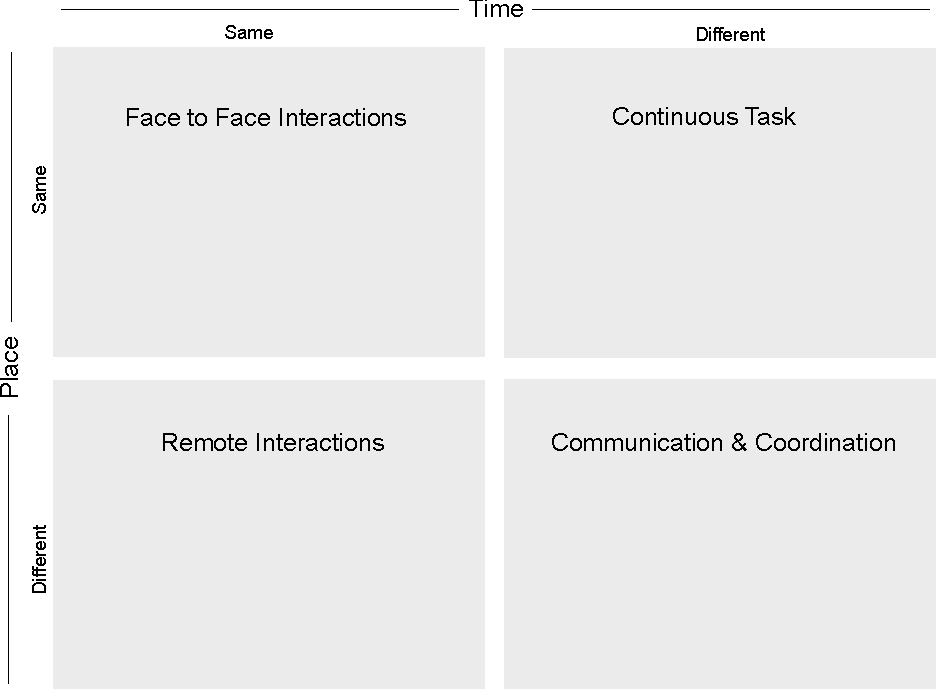
\includegraphics[width=0.8\columnwidth]{images/cscw_time_place_matrix.pdf}
 \caption[CSCW Place/Time Matrix]{\gls{CSCW} Place/Time Matrix \citep{xx}}
\label{fig:images_cscw_time_place_matrix}
\end{figure}

Additionally it is possible to group the CSCW systems based on the 3C model: \\

\begin{figure}[H]
 \centering
 %\includesvg[width=0.5\columnwidth, svgpath = images/]{cscw_time_place_matrix}
 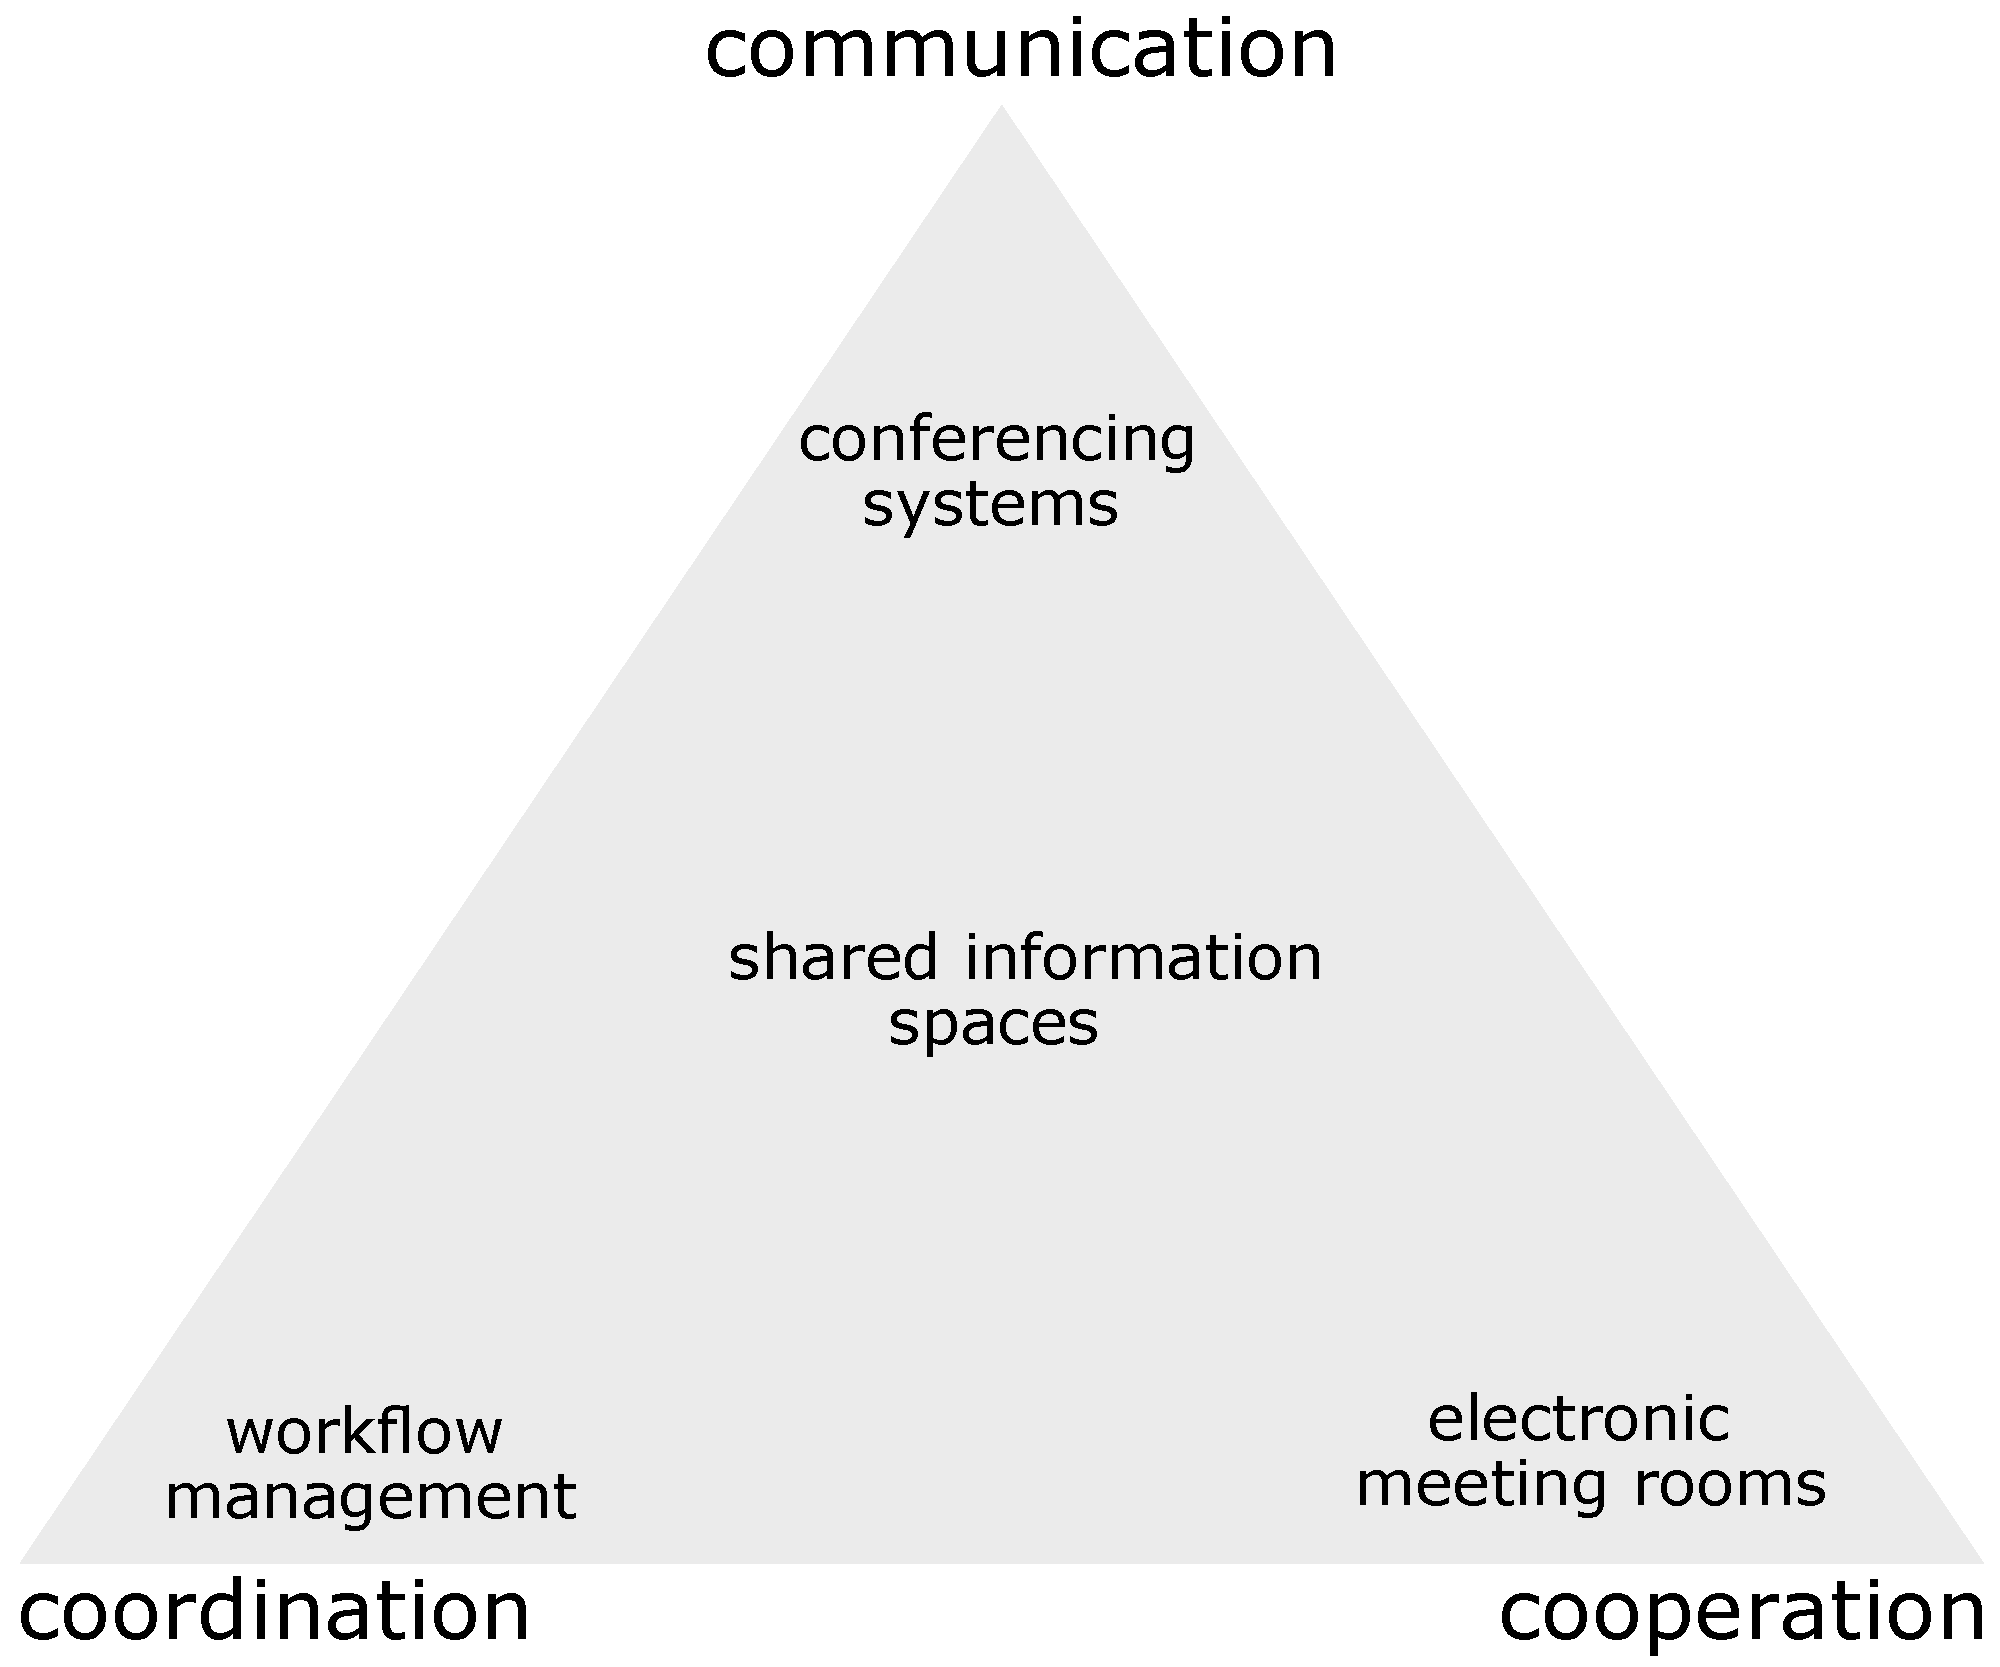
\includegraphics[width=0.8\columnwidth]{images/3C-model.pdf}
 \caption[The 3C Model]{The 3C Model \citep{Koch2008}}
\label{fig:images_cscw_3C_model}
\end{figure}

% section cscw_types (end)

\subsection{Shared Information Spaces}
\label{sec:cscw_shared_spaces}

% section cscw_shared_spaces (end)

\subsection{Important aspects of CSCW systems}
\label{sec:cscw_req_aspects}

% section cscw_req_aspects (end)

% section cscw (end)


% sub chapter semantic web
%!TEX root = ../MasterThesis.tex

\section{The Semantic Web}
\label{sec:semantic_web}

The \emph{Semantic Web} initiative strives for a better integration of distributed data from various publishers on the Web to enable new kinds of Smart Web applications. To achieve this goal, the Semantic Web delivers the infrastructure for this vision in form of various standard specifications such as \gls{RDF}, \gls{RDFS}, \gls{OWL}, \gls{SPARQL}, \ldots, which are introduced during the course of this section. Before going into the technical specifications of these the section shows the fundamental aspects underlying the (Semantic) Web as a whole.

\subsection{Fundamental aspects}
\label{subsec:fundamentals_semweb}

The Semantic Web builds on the fundamentals of the existing World-Wide Web, especially \citep[pg. 4-11]{allemang2011semantic}: \@

\begin{itemize}
	\item \textbf{AAA-Slogan:} Anyone can say Anything about Any topic. The Web does not restrict what people can post or publish on it. It is in the responsibilities of the readers to decide whether they can trust information from a specific source or not.
	\item \textbf{Open World Assumption:} as the amount of information on the Web is endless, and new information is published every day, one must always assume that there are new information available on it, that one does not know yet. As of this one can never be sure to have all facts at hand. New information can be published at any time that can give additional insights.
	\item \textbf{Non-unique Naming Assumption:} there is no central authority, who is responsible for providing unique identifiers for entities on the Web. Due to this fact different \gls{URI}s might refer to the same entity or real-world object.
\end{itemize}

Instead of making information on the Web available for human consumption \emph{only}, the Semantic Web is trying to make the information on the Web accessible (and readable) to machines as well. This will allow the integration of information across Web sites, and enable a distributed, interlinked ``Web of Data''. The major design principles to achieve this objective are \citep[pg. 1-22]{antoniou2008semantic}: \@

\begin{enumerate}
	\item make structured and semi-structured data available in standard formats,
	\item make individual data elements and their relationships accessible on the Web,
	\item describe the intended semantics of the data in a machine readable format
\end{enumerate}

The data model of the Semantic Web is build upon labeled graphs with objects and their relationships. Objects are modeled as nodes and their relationships as edges between them. To express these graphs of objects and their relationships, the Semantic Web: \@

\begin{itemize}
	\item formalize the syntax of the graph in \gls{RDF} (see Section~\ref{sec:semantic_rdf}),
	\item use \gls{URI}s to identify individual data items and relations (see Section~\ref{subsec:uri_concept}),
	\item use ontologies to represent semantics of the entities. Ontologies can be lightweight \gls{RDFS} definitions or expressive descriptions in the \gls{OWL} language (see Section~\ref{sec:semantic_ontologies}).
\end{itemize}

Initially it was tried to solve the data integration aspect on the Web with the exchange of \gls{XML} based messages, but though the \gls{XML} format is more machine-readable as \gls{HTML} it still lacks the semantic of the data transmitted (see Section~\ref{subsec:xml_format}). Therefore the Semantic Web defines the \gls{RDF} format as the basic data exchange format of it. Still the \gls{RDF} format was initially based on the \gls{XML} specification. To formally describe the existing terms and their relationships within a domain the Semantic Web relies on an ontology specification. These specifications are either expressed in \gls{RDFS} or uses the more expressive \gls{OWL} language; both of them are meta-description languages, which allows the definition of domain-specific knowledge representations based on the concepts found in \gls{RDF} itself. \\

As such the Semantic Web is a layered approach as depicted in Figure~\ref{fig:images_semweb_model}.\@

\begin{figure}[H]
	\centering
		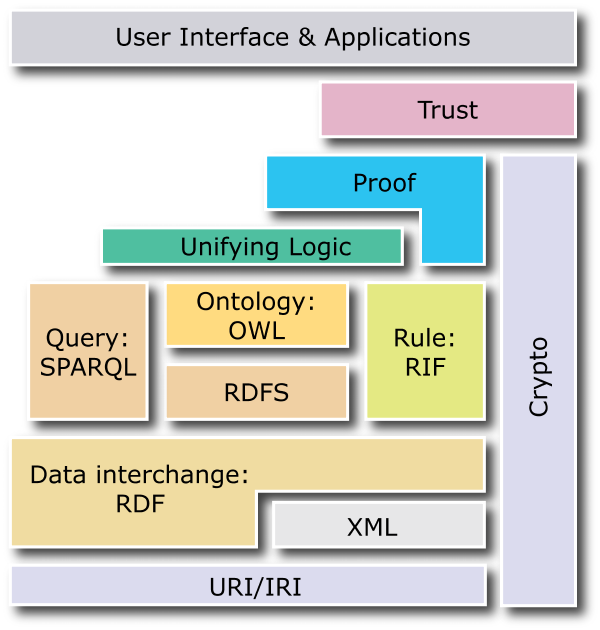
\includegraphics[width=0.8\columnwidth]{images/semantic_web_layers.png}
	\caption[The Semantic Web Model]{The Semantic Web Model \citep{W3C2013}}
\label{fig:images_semweb_model}
\end{figure}

% section semantic_fundamentals (end)

\subsection{Resource Description Framework}
\label{sec:semantic_rdf}

When trying to come up with a specification on how to integrate data on a globally dispersed platform such as the World-Wide Web, one will have to answer the following questions first: \@

\begin{itemize}
	\item \textbf{syntax:} How to serialize the data?
	\item \textbf{data model:} How to structure and organize the data?
	\item \textbf{semantics:} How to interpret the data?
\end{itemize}

Whereas the World-Wide Web is made up from interlinked documents in the \gls{HTML} format that is specifically designed for rendering information on screen to be consumed by a human, the \gls{RDF} brings a highly flexible data model to the Web. Its basic building block is the \emph{triple}, that is a statement consisting of an entity, an attribute and a value. The parts of a statement are also known as subject, predicate and object, which make up a directed graph as shown in the example in Figure~\ref{fig:images_semweb_triple}: \@

\begin{figure}[H]
	\centering
		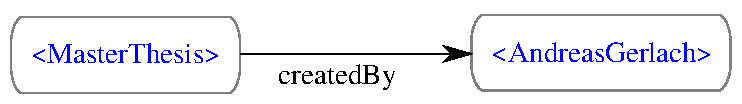
\includegraphics[width=0.8\columnwidth]{images/sample_triple.pdf}
	\caption{A basic example for a triple-statement}
\label{fig:images_semweb_triple}
\end{figure}

In this example the triple consists of the entity ``MasterThesis'', the assigned attribute ``createdBy'' and the value ``AndreasGerlach''. The value-part of a triple can contain either a literal value or another entity (as in the example above). Still a problem with this example statement is that the entities are not unique. Based on the given information it is not clear, which specific ``MasterThesis'' is meant and to whom the value ``AndreasGerlach'' refers. Additionally the predicate shown could have multiple meanings. These ambiguities have to be resolved on the Semantic Web to be able to make these information understandable by machines. To solve these issues the Semantic Web standard specifies that names of entities and predicates have to use a \gls{URI} (see Section~\ref{subsec:uri_concept}) to make their meanings clear. Literals that can be used as values such as numbers, dates and strings borrow their data type specifications from the \gls{XML} standard \citep[pg. 15-38]{wood2014linked}. \\

Based on this description the foundational elements of \gls{RDF} can be summarized as: \@

\begin{itemize}
	\item \textbf{entities:} aka resources or ``things'' of interest that are identified via \gls{URI}s
	\item \textbf{predicates:} aka attributes or properties that specify the relations between resources and are also identified by \gls{URI}s
	\item \textbf{literals:} integral values such as numbers, dates and strings that are based on the \gls{XML} data type specification
	\item \textbf{statements:} assign a value (either another entity or a literal) to a ``entity-predicate'' relation
	\item \textbf{graphs:} as the data model behind \gls{RDF} enables a  distributed, interlinked ``Web of Data''
\end{itemize}

\gls{RDF} triples can be serialized into four different syntax formats \citep[pg. 43-54]{wood2014linked}: \@

\begin{itemize}

	\item \textbf{\gls{RDF}/\gls{XML}:} the original format of the \gls{RDF} specification is based on the \gls{XML} specification. Because of their complexity they are best used with a parser program. For an example see Listing~\ref{lst:xml_meta_data}.
	\item \textbf{\gls{RDFa}:} describes how to embed \gls{RDF} information into existing \gls{HTML} documents. It allows Web site authors to enrich their Web pages with semantic information by adding a set of \gls{HTML} attributes to important items of the document. For an example see Listing~\ref{lst:rdfa_meta_data}.
	\item \textbf{\gls{JSON-LD}:} a recent initiative to allow JavaScript developers to use \gls{JSON} documents to express a \gls{RDF} statement, see Listing~\ref{lst:jsonld_meta_data}
	\item \textbf{Turtle:} a human readable serialization format for \gls{RDF} statements. \gls{URI}s can be shortened with a declared prefix, statements have to be finished with `.'. Statements referring to the same entity can be abbreviated via `;', which repeats the subject from the previous statement, or `,', which repeats subject and predicate from it. For an example see Listing~\ref{lst:turtle_meta_data}.
\end{itemize}

\begin{listing}[H]
	\begin{minted}[linenos,
	               numbersep=5pt,
	               breaklines=true,
	               frame=lines,
								 gobble=2]{XML}
		<?xml version="1.0"?>
		<rdf:RDF xmlns:rdfs="http://www.w3.org/2000/01/rdf-schema#"
			xmlns:ex="http://www.example.com/">
		  <rdf:Description rdf:about="http://www.example.com/MasterThesis">
		    <ex:createdBy rdf:resource="http://www.example.com/AndreasGerlach" />
		  </rdf:Description>
		</rdf:RDF>
	\end{minted}
\caption{A triple statement expressed in \gls{RDF}/\gls{XML} format}
\label{lst:xml_meta_data}
\end{listing}

\begin{listing}[H]
	\begin{minted}[linenos,
	               numbersep=5pt,
	               breaklines=true,
	               frame=lines,
								 gobble=2]{HTML}
	  <div about="http://www.example.com/MasterThesis">
	    <span rel="http://www.example.com/createdBy" resource="http://www.example.com/AndreasGerlach">
	  </div>
	\end{minted}
\caption{A triple statement expressed in \gls{RDFa} format}
\label{lst:rdfa_meta_data}
\end{listing}

\begin{listing}[H]
	\begin{minted}[linenos,
	               numbersep=5pt,
	               breaklines=true,
	               frame=lines,
								 gobble=2]{JSON}
  {
   "@context": "http://www.example.com/",
   "@id": "http://www.example.com/MasterThesis",
   "createdBy": "http://www.example.com/AndreasGerlach"
 	}
	\end{minted}
\caption{A triple statement expressed in \gls{JSON-LD} format}
\label{lst:jsonld_meta_data}
\end{listing}

\begin{listing}[H]
	\begin{minted}[linenos,
	               numbersep=5pt,
	               breaklines=true,
	               frame=lines,
								 gobble=2]{TURTLE}
	  @prefix ex:  <http://www.example.com/> .
	  ex:MasterThesis ex:createdBy ex:AndreasGerlach .
	\end{minted}
\caption{A triple statement expressed in Turle format}
\label{lst:turtle_meta_data}
\end{listing}

Coming back to the initial questions that have to be solved for data integration on a larger scale, this section showed how the Semantic Web tries to solve them, such as this: \@

\begin{itemize}
	\item \textbf{syntax:} supports the following formats: Turtle, \gls{RDFa}, \gls{RDF}/\gls{XML} and \gls{JSON-LD},
	\item \textbf{data model:} graph-based data model in \gls{RDF} specification,
	\item \textbf{semantics:} express semantics of the data in \gls{RDFS}. This will be the topic of the next section.
\end{itemize}

% section semantic_rdf (end)

\subsection{Web Ontologies}
\label{sec:semantic_ontologies}

Lightweight approach: RDFS \\
- is about adding semantics to your RDF documents \\
\\
Start by: \\
1. specify the \textbf{things} to talk about \\
   differentiate between \textit{objects} (real entities) and \textit{classes} (set of entities) \\
   `rdf:type' attribute to assign objects to classes (object = instance of this class) \\
   impose restrictions on the kind of properties used on objects: \\
   - restrictions on values are called `range' restrictions (object can take values of \ldots) \\
   - restrictions on property-object relations are called `domain' restrictions (this relation applies to objects of \ldots) \\
2. set up relations between classes (inheritance, composition) \\
3. define properties (registered globally) and the possible hierarchy relationship between them (global properties means you can
extend existing RDFS classes with your own properties easily) \\
\\
\begin{figure}[H]
	\centering
		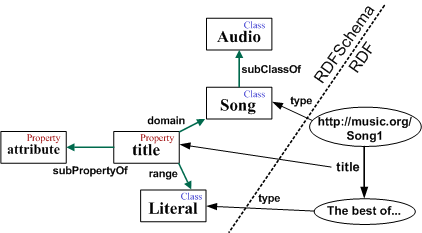
\includegraphics[height=2.5in]{images/RDFSchema.png}
	\caption{RDF Schema sample}
\label{fig:images_rdfs_sample}
\end{figure}

RDFS is described in RDF style using: \\
- core classes like: \\
  - `rdfs:Resource' (all objects/resources) \\
  - `rdfs:Class' (all classes) \\
  - `rdfs:Literal' (all literals) \\
  - `rdfs:Property' (all properties) \\
  - `rdfs:Statement' (all reified statements) \\
- core properties like: \\
  - `rdfs:type' (specify kind of class) \\
  - `rdfs:subClassOf' (specify inheritance between classes) \\
  - `rdfs:subPropertyOf' (specify inheritance between properties) \\
  - `rdfs:domain' (specify domain restrictions) \\
  - `rdfs:range' (specify range restrictions) \\
- container classes like: \\
  - `rdf:Bag'  (unordered list of entitites) \\
  - `rdf:Seq'  (ordered list of entities) \\
  - `rdf:Alt'  (list of alternatives/choices) \\
  - `rdf:Container' (superclass for all containers) \\
- utility classes like: \\
  - `rdfs:seeAlso', `rdfs:isDefinedBy' (links and references to other entities) \\
  - `rdfs:Comment' (comments and notes of entities) \\
  - `rdfs:Label' (human-friendly name of entities) \\
\\

Missing features in RDFS: \ldots  \\
\\
Complex Ontologies in Web Ontology Language (OWL): \\
\ldots \\
\\

% section semantic_ontologies (end)

\subsection{Query Language}
\label{sec:semantic_querylang}

SPARQL requires a \textbf{triple store} - a database containing RDF documents \\
is also referred to as a \textit{Graph Store} \\
data is inserted via Bulk load operation or via SPARQL update statements \\
SPARQL consist of SPARQL Queries that are send over the SPARQL protocol \\
Clients sends the queries to an HTTP endpoint \\
Stores on the public Web incl. dbpedia.org, ckan.org, wikidata.org \\
SPARQL also works with RDFS \\
SPARQL has similarities to SQL:
- each element in a triple might be replaced with a variable like `?varName' like so: \\

\begin{listing}[H]
	\begin{minted}[linenos,
	               numbersep=5pt,
	               gobble=2,
	               frame=lines,
	               framesep=2mm]{SPARQL}
	  PREFIX ns1:<URI>
	  PREFIX ns2:<URI>
	  PREFIX ns3:<URI>

	  SELECT ?varName
	  WHERE {
	      ns1:subject ns2:predicate ?varName
	  }
	\end{minted}
\caption{Selecting information with \gls{SPARQL}}
\label{lst:select_sparql}
\end{listing}

- in the WHERE clause it hosts the graph pattern to match (could be cascaded to go down subgraphs) \\
- variables can occur at any place in the graph pattern (?subj ?pred ?obj) as select with query everything \\
\\
LIMIT \textless n\textgreater option at the end for limiting the result set \\
FILTER (?varName \textless condition\textgreater ) in graph pattern can restrict results to match some
literal values and supports: \\
- numbers, dates: \textless, \textgreater, = \\
- strings: =, regex() \\
\\
\textbf{open world} assumption: resources on the Web are described in different schematas with various properties
using different vocabularies \\
- UNION option in graph pattern combines different matches \\
- OPTIONAL option in graph pattern only returns those entities if they are available (otherwise empty) \\
\\
ASK query checks for the existence of a given graph pattern \\
CONSTRUCT can be used to retrieve a subgraph from a larger graph, can also be used to translate between different schemas \\

\begin{listing}[H]
	\begin{minted}[linenos,
	               numbersep=5pt,
	               gobble=2,
	               frame=lines,
	               framesep=2mm]{SPARQL}
	  PREFIX ns1:<URI>
	  PREFIX ns2:<URI>
	  PREFIX ns3:<URI>

	  CONSTRUCT {
	      ?varA ns2:predicate ?varB .
	      ?varA ns3:predicate ?literalA .
	  }
	  WHERE {
	      ?varA ns1:predicate ?varB
	  }
	  FILTER ( ?varB > x )
	\end{minted}
\caption{A CONSTRUCT query in \gls{SPARQL}}
\label{lst:construct_sparql}
\end{listing}

- SPARQL can be used to harmonize graphs from different sources \\
- is also used for basic reasoning ala ``if found this, assume that'' \\
- can ease hierarchical queries with * or + on the predicate (SPARQL 1.1) \\
- can help resolving issues with different entities referring to the same object (MKP pg. 95)\\
- Federated Queries can be used to combine information from distinct sources via SPARQL (MKP pg. 110-112)\\
\\
- inferencing information from existing triples via SPIN (SPARQL Inferencing Notation) \\
- like in a taxonomy items can be categorized in an hierarchy (MKP pg. 114) \\
- inference patterns are used in Semantic Web applications (MKP pg. 115) \\
   * subClassOf - type propagation rule \\
- inferencing could be done at query time or persistently (MKP pg. 120/121) \\
- inferences can also be helpful when combining information from unknown sources \\
- inferencing happens on various levels (RDFS, RDFS+, OWL) with an increased set of complex inferencing rules (MKP pg. 122/123)
\\
% section semantic_querylang (end)

\subsection{Agents and Rules}
\label{sec:semantic_logic_rules}


% section semantic_logic_rules (end)

% section semantic_web (end)


% sub chapter peer-to-peer communications
%!TEX root = ../MasterThesis.tex

\section{Peer-to-peer communication}
\label{sec:p2p_communication}

This section explains the core concepts of \gls{P2P} communication technologies. It begins with a comparison of the benefits and disadvantages of centralized and decentralized Web architectures. After that it shows how \gls{P2P} communication networks can be structured, the different ways to initiate a communication session as well as how data can be transmitted between peers.

\subsection{Centralized vs. Decentralized Web architectures}
\label{sec:central_decentral_arch}

In classical client-server applications the information is stored on a central system (aka server). Clients have to connect to the server and ask for the information. The server handles the requests from the clients and deliver the information in case a request was valid. Prominent examples of centralized Web architectures are Social Networks such as Facebook or Twitter, in which clients, such as a Web browser or Mobile application, communicate with a Web service that runs on a server of the organization providing these Social Networks, to access and retrieve Web documents (e.g.\ \gls{HTML}, images, audio, video, \ldots) via the \gls{HTTP} protocol, as shown in Figure~\ref{fig:p2p_central_server}. \@

\begin{figure}[H]
	\centering
		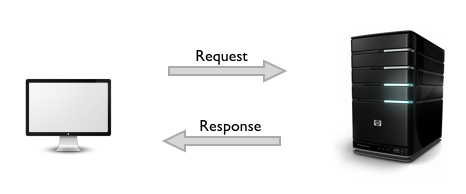
\includegraphics[width=0.9\columnwidth]{images/client-server-web.png}
	\caption[Centralized Web architectures as used by prominent Social Networks]{Centralized Web architectures as used by prominent Social Networks \citep{codeTuts}}
\label{fig:p2p_central_server}
\end{figure}

As a consequence of this architecture all of the information are centralized and under control of the provider of the (Web) service. This can lead to a variety of problems, including serious issues such as unreliable or no longer existing services will result in a dismissal of all the information stored on them, or privacy concerns for user-generated content stored on those central servers. \\

In opposite to that a \gls{P2P} network considers all nodes as equal. This offers the benefits that information can be kept on each node, and each node can provide access to its information to any other node on the network. Due to this the \gls{P2P} system has an high degree of decentralization, is not owned and controlled by a specific company, and therefore tends to me more resilient to faults, outages and attacks. But due to the distributed nature of it, looking for and accessing information is more difficult. Information in a \gls{P2P} system have to be indexed in a way so that the correct node is queried for it. Still this index has to be stored somewhere in the system, and the optimal solution for the indexing problem depends on the type of \gls{P2P} system used (see next section). Additionally, the way new nodes get connected to the system is depending on the type of \gls{P2P} system used, and might lead to the introduction of special bootstrap or super nodes into the network as shown in Figure~\ref{fig:p2p_overlay_network} \citep{parameswaran2001p2p}.

\begin{figure}[H]
	\centering
		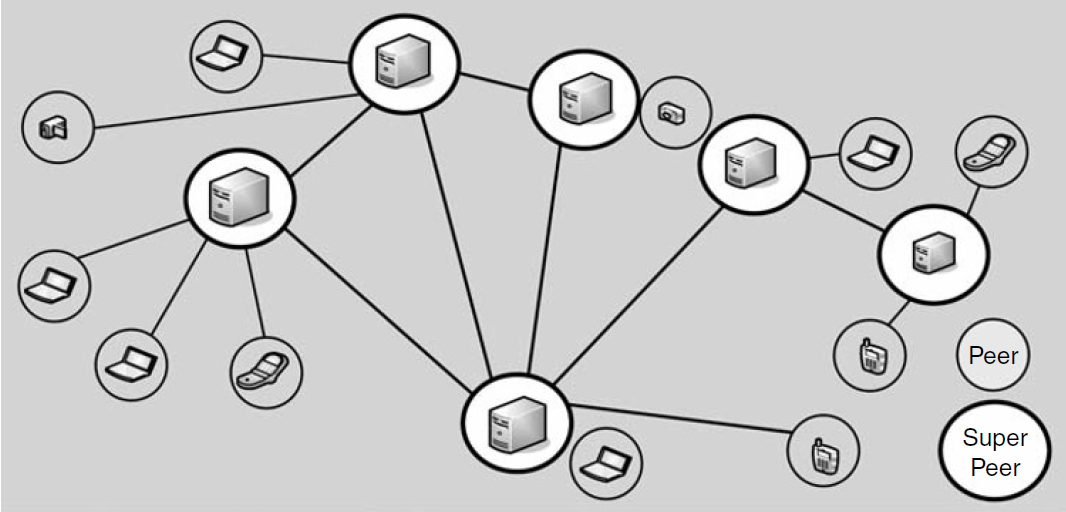
\includegraphics[width=0.8\columnwidth]{images/p2p_network.png}
	\caption[A \gls{P2P} overlay network]{A \gls{P2P} overlay network \citep[pg. 9]{buford2009p2p}}
\label{fig:p2p_overlay_network}
\end{figure}

% section central_decentral_arch (end)

\subsection{Classification of \gls{P2P} systems}
\label{sec:p2p_classification}

\gls{P2P} system architectures can be classified based on their degree of centralization into: \@

\begin{itemize}
	\item \textbf{partially centralized \gls{P2P} system:} rely on a dedicated controller node that maintains the set of participating nodes, host the index of the information available in the system, and controls the overall operation of the network,
	\item \textbf{decentralized \gls{P2P} system:} does not use any dedicated controller node, but may need to introduce bootstrap and super nodes for maintaining the list of participating nodes and the index of the information available depending on the size of the network.
\end{itemize}

\begin{figure}[H]
	\centering
		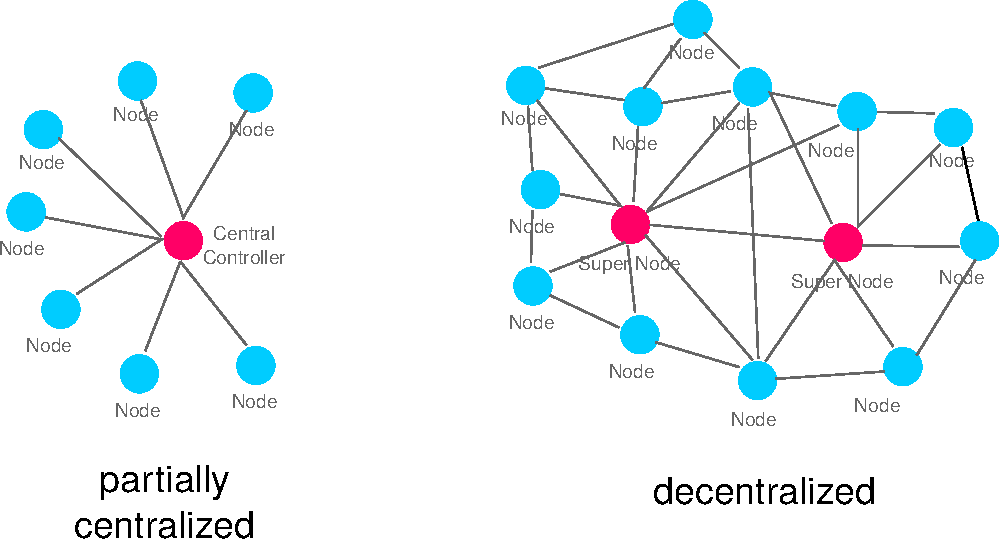
\includegraphics[width=0.8\columnwidth]{images/p2p_network_structures.pdf}
	\caption{Classification of \gls{P2P} networks}
\label{fig:p2p_network_structures}
\end{figure}

% section p2p_classification (end)

\subsection{Communication in a \gls{P2P} network}
\label{sec:p2p_start_communication}

The procedure to establish a \gls{P2P} communication depends on the structure of the \gls{P2P} system. In a \emph{partly centralized \gls{P2P} system} new nodes join the network by connecting to the central controller first. This central controller has a well-known \gls{IP} address and maintains the operation of the whole \gls{P2P} network. Due to this, any new node has to register with the central controller to get introduced to the \gls{P2P} network. The controller also maintains the information about the overlay network as well as the information about each object and on which node(s) it resides within the network. The overlay is typically following a star-shaped topology with the central controller at the center, see Figure~\ref{fig:p2p_network_structures}. \\

In a \emph{decentralized \gls{P2P} system} new nodes are expected to obtain the \gls{IP} address they have to connect to initially via a separate channel (e.g.\ as a link on a Web site). Depending on the size of the \gls{P2P} network additional bootstrap or super nodes, which help to set up a new node, are available on the network. These special nodes are generally also consolidating information about the objects available on the peers nearby, which helps speeding up searching and accessing required information. The overlay information of such a distributed network can be either \emph{structured}, in which each node receives a unique identifier from a numeric keyspace resembling the responsibilities of that node, or \emph{unstructured}, in which there is no particular network structure, and no further constraints are assigned to the nodes of the network. \\

A \emph{structured overlay} maintain the information within the network more efficiently, because it uses a distributed hash-table to maintain a distributed index and decides the location (aka node) of an object in the network based on its hash-value. In an \emph{unstructured overlay network} the information is typically stored on the node that introduces it. To locate an object a query request is typically broadcasted through the overlay network. Based on the size of the network and the distance between the node asking for and the node holding the information querying and accessing an information on an unstructured overlay network can take some time, and can also flood the whole network with query requests. Therefore, requesting nodes often set the scope of the request, which limits the number of hops that should be done on the network. This will reduce the communication overhead on the whole system. Additionally, introducing super nodes that collect and maintain indexes of their peers nearby can further reduce the number of hops necessary to find the required information, see Figure~\ref{fig:p2p_network_structures} \citep{rodrigues2010peer}. \@

% section p2p_start_communication

\subsection{The \gls{WebRTC} standard}
\label{sec:p2p_webrtc}

``Web Real-Time Communication (\gls{WebRTC}) is a collection of standards, protocols, and JavaScript \gls{API}s, the combination of which enables peer-to-peer audio, video, and data sharing between browsers (peers)'' \citep[pg. 307]{grigorik2013high}. Although this new \gls{W3C} standard usually stands for in-browser video or audio conferencing without the need of proprietary browser extensions, it also offers ways to exchange arbitrary messages or binary data between participating peers in a distributed Web application. Due to being an open Web standard \gls{WebRTC} is available in many current Web browsers directly, and is widely adopted as a standardized and open way to establish a \gls{P2P} communication between clients of a Web site, or from within a Web application. The standard wraps a lot of the complexities of establishing peer-to-peer communication channels and transmitting data into three primary \gls{API}s \citep[pg. 307-308]{grigorik2013high}: \@

\begin{itemize}
	\item \textbf{MediaStream:} for acquiring access to and retrieve data from local audio and video devices,
	\item \textbf{RTCPeerConnection:} for establishing a peer-to-peer connection between clients,
	\item \textbf{RTCDataChannel:} for transmitting arbitrary application data
\end{itemize}

To establish a data connection between peers a Web application has to create a RTCPeerConnection object first, before it can create a RTCDataChannel to exchange messages on it. Establishing a \gls{P2P} connection between globally dispersed peers on the Web is not a trivial task and has to provide fallback solutions in case of \gls{P2P} connectivity issues due to firewall or \gls{NAT} services used by some of the peers, which usually prevent clients to connect to each other directly. Fortunately, the \gls{W3C} standard is taking care of these steps during the initiating of a \gls{WebRTC} connection by utilizing the \gls{ICE} protocol. After being able to open a connection to another peer, a communication session has to be created. For that the communicating peers have to negotiate on protocols, encodings, and additional functionality required for the \gls{P2P} communication tasks at hand. The \gls{WebRTC} uses the \gls{SCTP} to exchange application data between peers \citep[pg. 315-330]{grigorik2013high}. It has the following set of features \citep[pg. 342]{grigorik2013high}: \@

\begin{itemize}
		\item \textbf{Reliability:} the data channel can be configured to use either reliable or unreliable delivery of packages,
		\item \textbf{Delivery:} the data channel can be also configured to support either in-order or out-of-order delivery of packages,
		\item \textbf{Transmission:} the transport of data is message-oriented,
		\item \textbf{Confidentiality/Integrity:} all application data transmitted between the peers is encrypted to guarantee confidentiality and integrity of the data exchanged.
\end{itemize}

For a purely data transmission channel one can also disable any audio and video transfers during the setup of the communication session (see Listing~\ref{lst:p2p_webrtc_data_only}). \@

\begin{listing}[H]
	\inputminted[linenos,
							 numbersep=5pt,
							 breaklines=true,
							 frame=lines]{JavaScript}
		{./samples/initiateWebRTCConnection.js}
\caption[Establishing a pure \gls{WebRTC} data connection]{Establishing a pure \gls{WebRTC} data connection \citep[pg. 349]{grigorik2013high}}
\label{lst:p2p_webrtc_data_only}
\end{listing}

Once a data channel has been established between the peers application data can be exchanged between them via message passing, as shown in Listing~\ref{lst:p2p_webrct_data_send}: \@

\begin{listing}[H]
	\inputminted[linenos,
							 numbersep=5pt,
							 breaklines=true,
							 frame=lines]{JavaScript}
		{./samples/handleWebRTCDataChannel.js}
\caption[Message-oriented communication via a \gls{WebRTC} data channel]{Message-oriented communication via a \gls{WebRTC} data channel \citep[pg. 346]{grigorik2013high}}
\label{lst:p2p_webrct_data_send}
\end{listing}

% section p2p_webrtc (end)

% section p2p_communication (end)


% chapter theoretical foundations (end)
